%! TeX program = lualatex
\documentclass[../main.tex]{subfiles}

\usetikzlibrary{intersections,calc}

\newenvironment{solution}{
  \begin{proof}[Sample solution]
    \color{main}
  }{
  \end{proof}
}

\begin{document}

\chapter*{Week 6 practice problems}

\setcounter{chapter}{6}

\begin{example}
  Toss a coin and roll a four-sided die labelled \(1,2,3,4\).  Find the probability of getting a tail and an even number.

  \begin{solution}
    The sample space is 
    \[
      \{ H1, H2, H3, H4, T1, T2, T3, T4 \}.
    \]

    The event is \(\{ T2, T4 \}\). So the probability is \(2/8\).
  \end{solution}
\end{example}

\begin{exercise}
  Let \(A = \{3,7,9,17,48\}\) and \(C = \{2,7,8,13\}\) be two events. List the outcomes in \(A \cup C\). How many outcomes are in \(A \cup C\)?

  \begin{solution}
    Note \(A \cup C = \{ 3,7,9,17,48, 2,8,13 \}\). Notice the \(7\) appears in both events but is \emph{not} duplicated.  There are \(8\) outcomes in \(A \cup C\).
  \end{solution}
\end{exercise}


\begin{exercise}
  Shade the events \((A \cap B^{c}) \cup C^{c}\) and \(A^{c} \cap (B \cup C)^{c}\).
  
  \begin{center}
    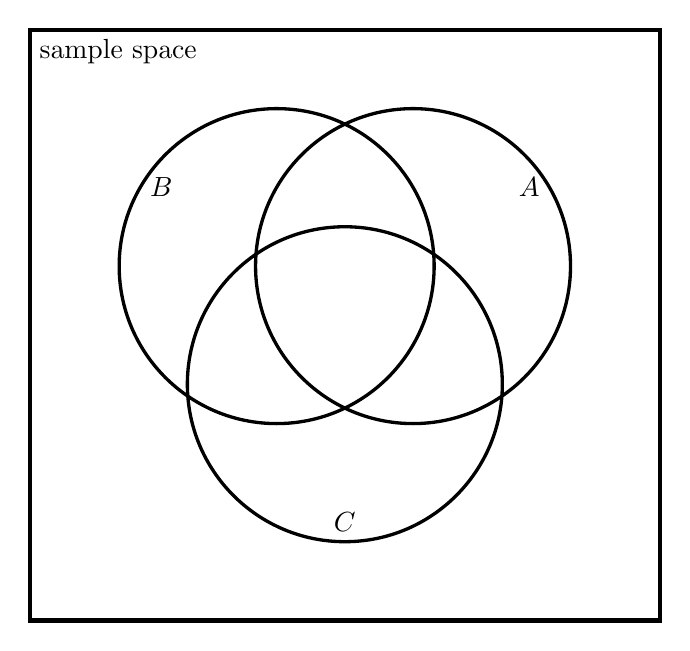
\begin{tikzpicture}
      \draw[ultra thick] (-4,-4) rectangle (4,3.5);
      \node[below right] at (-4,3.5) {sample space};

      \draw[very thick] ( 30:1) circle[radius=2];
      \draw[very thick] (150:1) circle[radius=2];
      \draw[very thick] (-90:1) circle[radius=2];
      \node[left]  at ( 30:3) {\(A\)};
      \node[right] at (150:3) {\(B\)};
      \node[above] at (-90:3) {\(C\)};
    \end{tikzpicture}
    \quad
    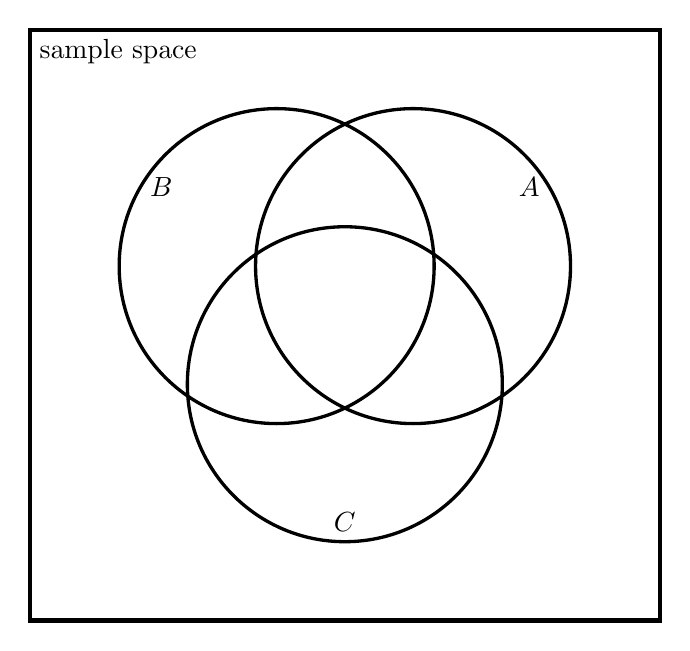
\begin{tikzpicture}
      \draw[ultra thick] (-4,-4) rectangle (4,3.5);
      \node[below right] at (-4,3.5) {sample space};

      \draw[very thick] ( 30:1) circle[radius=2];
      \draw[very thick] (150:1) circle[radius=2];
      \draw[very thick] (-90:1) circle[radius=2];
      \node[left]  at ( 30:3) {\(A\)};
      \node[right] at (150:3) {\(B\)};
      \node[above] at (-90:3) {\(C\)};
    \end{tikzpicture}
  \end{center}

  \pagebreak
  \begin{solution}
  The event \((A \cap B^{c}) \cup C^{c}\) is shown on the left and \(A^{c} \cap (B \cup C)^{c}\) on the right.

  \begin{center}
    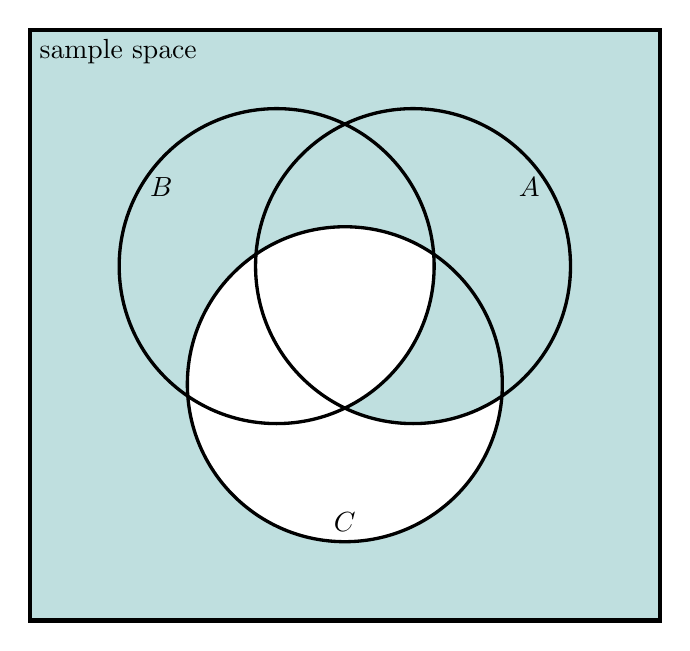
\begin{tikzpicture}
      %--- circles A (right), B (left), C (bottom)
      \def\R{2}
      \path ( 30:1) coordinate (Acenter);
      \path (150:1) coordinate (Bcenter);
      \path (-90:1) coordinate (Ccenter);

      %==================== SHADING ====================

      % 1) Shade C^c : the rectangle minus circle C (even-odd rule)
      \fill[teal!25, even odd rule]
        (-4,-4) rectangle (4,3.5)
        (Ccenter) circle[radius=\R];

      % 2) Shade (A ∩ C ∩ B^c):
      %    First fill A ∩ C, then remove the triple intersection A ∩ B ∩ C.
      %    (This leaves A ∩ C minus B.)
      \begin{scope}
        \clip (Acenter) circle[radius=\R];
        \clip (Ccenter) circle[radius=\R];
        \fill[teal!25] (-4,-4) rectangle (4,3.5); % fills A ∩ C
      \end{scope}
      % remove A ∩ B ∩ C from the previous fill to get B^c
      \begin{scope}
        \clip (Acenter) circle[radius=\R];
        \clip (Bcenter) circle[radius=\R];
        \clip (Ccenter) circle[radius=\R];
        \fill[white] (-4,-4) rectangle (4,3.5); % subtracts A ∩ B ∩ C
      \end{scope}

      %==================== OUTLINES ====================
      \draw[black, very thick] (Acenter) circle[radius=\R];
      \draw[black, very thick] (Bcenter) circle[radius=\R];
      \draw[black, very thick] (Ccenter) circle[radius=\R];

      \node[black, left]  at  ( 30:3) {\(A\)};
      \node[black, right] at  (150:3) {\(B\)};
      \node[black, above] at (-90:3) {\(C\)};

      \draw[black, ultra thick] (-4,-4) rectangle (4,3.5);
      \node[black, below right] at (-4,3.5) {sample space};
    \end{tikzpicture}
    \quad
    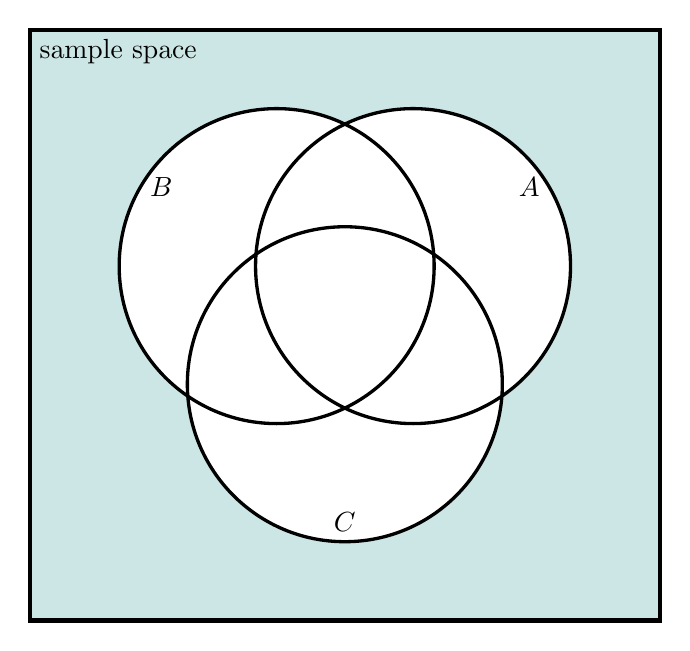
\begin{tikzpicture}
      % Shade (A ∪ B ∪ C)^c
      \fill[teal!20, even odd rule]
        (-4,-4) rectangle (4,3.5)
        (30:1) circle[radius=2]
        (150:1) circle[radius=2]
        (-90:1) circle[radius=2];

      \fill[white] (0,0) circle[radius={2.3}];

      % Circles
      \draw[black, very thick] (30:1) circle[radius=2];
      \draw[black, very thick] (150:1) circle[radius=2];
      \draw[black, very thick] (-90:1) circle[radius=2];

      % Labels
      \node[black, left]  at (30:3) {\(A\)};
      \node[black, right] at (150:3) {\(B\)};
      \node[black, above] at (-90:3) {\(C\)};

      % Sample space
      \draw[black, ultra thick] (-4,-4) rectangle (4,3.5);
      \node[black, below right] at (-4,3.5) {sample space};
    \end{tikzpicture}
  \end{center}
  \end{solution}
\end{exercise}

\begin{exercise}
  Suppose the sample space is \(\Omega = \{1,2,3,4,5\}\).  Let \(E = \{2,5\}\), \(F = \{1,2,3\}\) and \(G = \{2,4\}\). Find the probability \(\mathbb{P}( (E \cap G^{c}) \cap ( F^{c} \cup E^{c} )) \).

  \begin{solution}
    We break the problem into two little problems. List \(E \cap G^{c} = \{ 5 \}\) and \(F^{c} \cup E^{c} = \{ 4,5, 1,3\}\). Now we see \(\left( E \cap G^{c} \right) \cap \left( F^{c} \cup E^{c} \right) = \{5\}\). So the probability is \(1/5\).
  \end{solution}
\end{exercise}

\begin{exercise}
  Suppose \(A = \{1\}, B = \{1,2,4\}, C = \{1,3,5\}\) are events in a sample space \(\Omega = \{1,2,3,4,5\}\). Calculate \(\mathbb{P}( (A \cup B)^{c} \cap C^{c} )\).

  \begin{solution}
    Notice \(A \cup B = \{ 1,2,4\}\), so \((A \cup B)^{c} = \{3,5\}\).  Then \((A \cup B)^{c} \cap C^{c}\) is empty. Therefore, the probability is \(0\).
  \end{solution}
\end{exercise}

\begin{exercise}
  Suppose the sample space is \(\Omega = \{1,2,\ldots,10\}\).  Let \(E = \{1,3,5\}\) and \(F = \{2,7,3,4\}\). Find the probability \(\mathbb{P}( (E \cap F) \cup (E \cap F^{c})) \).

  \begin{solution}
    Notice \(E \cap F = \{ 3\}\) and \(E \cap F^{c} = \{1,5\}\). So \((E \cap F) \cup (E \cap F^{c}) = \{1,3,5\}\). Therefore, the probability is \(3/10\).
  \end{solution}
\end{exercise}

\begin{exercise}
  Suppose \(A,B\) are events in a common sample space. An intern calculated \(\mathbb{P}(A) = 9\%\), \(\mathbb{P}(A \cap B) = 7\%\) and \(\mathbb{P}(A \cup B) = 98\%\). Find \(\mathbb{P}(B)\).

  \begin{solution}
    Using the principle of inclusion-exclusion, we have \(\mathbb{P}(A \cup B) = \mathbb{P}(A) + \mathbb{P}(B) - \mathbb{P}(A \cap B)\). Isolate for \(\mathbb{P}(B)\), we get
    \[
      \mathbb{P}(B) = \mathbb{P}(A \cup B) + \mathbb{P}(A \cap B) - \mathbb{P}(A) = 98\% + 7\% - 9\% = 96\%.
    \]

  \end{solution}
\end{exercise}

\begin{exercise}
  Consider the days in March. Weather forecast predicts that there will be \(20\) sunny days, \(8\) snowy days, \(13\) windy days. Is there enough information to determine the probability of having a cold day given it is windy? If so, what is the probability?

  \begin{solution}
  No. The required probability is \(\mathbb{P}( \text{cold} \mid \text{windy} ) = \frac{\mathbb{P}(\text{cold} \cap \text{windy})}{\mathbb{P}(\text{windy})}\). However, we don't enough information to find \(\mathbb{P}(\text{cold} \cap \text{windy})\).
  \end{solution}
\end{exercise}

\begin{exercise}
  Suppose \(\mathbb{P}(E) = 0.2\), \(\mathbb{P}(F) = 0.5\) and \(\mathbb{P}(E \mid F) = 0.25\). Calculate \(\mathbb{P}(E \cap F)\).

  \begin{solution}
    The definition for a conditional probability is simply a relation
    \[
      \mathbb{P}(E \mid F) = \frac{\mathbb{P}(E \cap F)}{\mathbb{P}(F)}. 
    \]
    Rearrange we get  \(\mathbb{P}(E \cap F) = \mathbb{P}(E \mid F) \mathbb{P}(F) = 0.25 \times 0.5 = 0.125\).
  \end{solution}
\end{exercise}

\begin{exercise}
  A clothing store is stocked with \(95\) T-shirts, \(25\) jackets, \(15\) dress pants, \(40\) sweat pants and \(100\) socks. 
  What is the probability that a randomly selected pair of pants is a pair of sweat pants?

  \begin{solution}
    Note \(\mathbb{P}(\text{sweat pants} \mid \text{pants}) = \frac{\mathbb{P}(\text{sweat pants} \cap \text{pants})}{\mathbb{P}(\text{pants})} = \frac{40}{40 + 15}\).
  \end{solution}
\end{exercise}

\begin{exercise}
  A city of \(10000\) residents is offered a new blood‑based screening test for a certain illness.  Health officials already know from previous studies that \(1000\) of these residents actually have the disease. The rest do not.

  \begin{enumerate}
    \item Out of the \(1000\) residents who have the disease, the test correctly identifies \(920\) of them.
    \item Among the residents who do not have the disease, the test incorrectly labels 450 of them as positive.
  \end{enumerate}

  Calculate \(\mathbb{P}(\text{true positive})\), \(\mathbb{P}(\text{true negative})\), \(\mathbb{P}(\text{false positive})\) and \(\mathbb{P}(\text{false negative})\).

  \begin{solution}
    From the given data, we have a handy table.

    \begin{center}
      \begin{tabular}{l|c||c}
      & sick & not sick \\\midrule
        \(+\) & 920 & 450 \\\midrule
        \(-\) & & 
      \end{tabular}
    \end{center}

    The sick column should sum to \(1000\) and the not-sick column sums to \(9000\). We can now fill in the blanks.
    \begin{center}
      \begin{tabular}{l|c||c}
      & sick & not sick \\\midrule
        \(+\) & 920 & 450 \\\midrule
        \(-\) & 80 & 8550
      \end{tabular}
    \end{center}

    The probabilities are
    \begin{align*}
      \mathbb{P}(\text{true positive}) &= 920/100, \\
      \mathbb{P}(\text{false negative}) &= 80/1000, \\
      \mathbb{P}(\text{false positive}) &= 450/9000, \\
      \mathbb{P}(\text{true negative}) &=  8550/900.
    \end{align*}
  \end{solution}
\end{exercise}

\begin{exercise}
  A software monitors banking transactions for fraud. The software was tested using historical data with known fraudulent transactions. It produced a false negative rate of \(20\%\) but a true negative rate of \(97\%\). The prevalence of fraudulent transactions in the historical data is \(5\%\).
  
  \begin{enumerate}
    \item Calculate \(\mathbb{P}(\text{true positive})\), \(\mathbb{P}(\text{true negative})\), \(\mathbb{P}(\text{false positive})\) and \(\mathbb{P}(\text{false negative})\).
    \item Find the probability that a transaction is flagged as a fraud.
    \item If \(25\) million transactions were monitored by the software, how many flagged transactions are expected to be truly fraudulent?
  \end{enumerate}

  \begin{solution}
    We are directly given this information
    \begin{center}
      \begin{tabular}{l|c||c}
      & fraud & not fraud \\\midrule
        \(+\) &  & \\\midrule
        \(-\) & \(20\%\) & \(97\%\)
      \end{tabular}
    \end{center}

    Each column sums to \(100\%\). We just fill in the blanks.
    \begin{center}
      \begin{tabular}{l|c||c}
      & fraud & not fraud \\\midrule
        \(+\) & \(80\%\) & \(3\%\) \\\midrule
        \(-\) & \(20\%\) & \(97\%\)
      \end{tabular}
    \end{center} 

    \begin{enumerate}
      \item The probabilities are directly read off the table.
        \begin{align*}
          \mathbb{P}(\text{true positive}) &= 80\%, \\
          \mathbb{P}(\text{false negative}) &= 20\%, \\
          \mathbb{P}(\text{false positive}) &= 3\%, \\
          \mathbb{P}(\text{true negative}) &=  97\%.
        \end{align*}

      \item We can bypass any fancy formulas and think intuitively here. Since the prevalence is \(5\%\), if the software looks over \(Y\) number of transactions, then \(80\% \times 5\% Y\) are true positives, and \(3\% \times 95\% Y\) are false positives. Then
        \[
          \mathbb{P}(\text{positives}) 
          = \frac{80\% \times 5\% Y + 3\% \times 95\% Y}{Y}
          = 80\% \times 5\% + 3\% \times 95\%.
        \]

      \item We are asked to find the number of true positives. Since the prevalence is \(5\%\), there will be \(0.05 \times 25 = 1.25\) million fraudulent transactions. \(80\%\) of these will be flagged by the software. Therefore, \(80\% \times 1.25 = 1\) million flagged transactions are truly fraudulent.
    \end{enumerate}
  \end{solution}
\end{exercise}

\begin{exercise}
  A doctor's true positive rate for diagnosing osteoarthritis is \(99\%\).  If the doctor thinks a patient does not have osteoarthritis, is there enough data to support that the diagnose is likely to be correct?

  \begin{solution}
    True negatives and true positive are not related. There is not enough data to determine \(\mathbb{P}(\text{true negative})\).
  \end{solution}
\end{exercise}


\end{document}
